\hypertarget{group___i_r_c_interface_callbacks}{\section{Callbaks}
\label{group___i_r_c_interface_callbacks}\index{Callbaks@{Callbaks}}
}
Collaboration diagram for Callbaks\-:
\nopagebreak
\begin{figure}[H]
\begin{center}
\leavevmode
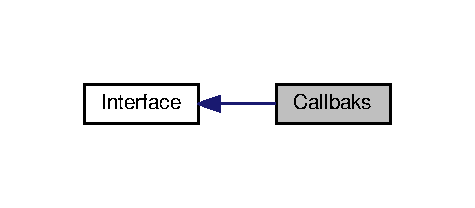
\includegraphics[width=228pt]{group___i_r_c_interface_callbacks}
\end{center}
\end{figure}
Funciones que van a ser llamadas desde el interface y que deben ser implementadas por el usuario. Todas estas funciones pertenecen al hilo del interfaz.

El programador puede, por supuesto, separar todas estas funciones en múltiples ficheros a efectos de desarrollo y modularización.



 \hypertarget{IRCInterface_ActivateChannelKey}{}\subsubsection{I\-R\-C\-Interface\-\_\-\-Activate\-Channel\-Key}\label{IRCInterface_ActivateChannelKey}
Llamada por el botón de activación de la clave del canal.


\begin{DoxyCode}
\textcolor{preprocessor}{#include <redes2/ircxchat.h>}

\textcolor{keywordtype}{void} \hyperlink{xchat2_8c_a33f80a29a744e4182b29e23f13c1f05c}{IRCInterface\_ActivateChannelKey} (\textcolor{keywordtype}{char} *channel, \textcolor{keywordtype}{char} * key)
\end{DoxyCode}


Llamada por el botón de activación de la clave del canal. El segundo parámetro es la clave del canal que se desea poner. Si es N\-U\-L\-L deberá impedirse la activación con la función implementada a tal efecto. En cualquier caso sólo se puede realizar si el servidor acepta la orden. Las strings recibidas no deben ser manipuladas por el programador, sólo leídas.


\begin{DoxyParams}[1]{Parameters}
\mbox{\tt in}  & {\em channel} & canal sobre el que se va a activar la clave. \\
\hline
\mbox{\tt in}  & {\em key} & clave para el canal indicado.\\
\hline
\end{DoxyParams}
\begin{DoxyWarning}{Warning}
Esta función debe ser implementada por el alumno.
\end{DoxyWarning}
\begin{DoxyAuthor}{Author}
Eloy Anguiano (\href{mailto:eloy.anguiano@uam.es}{\tt eloy.\-anguiano@uam.\-es})
\end{DoxyAuthor}


 \hypertarget{IRCInterface_ActivateExternalMessages}{}\subsubsection{I\-R\-C\-Interface\-\_\-\-Activate\-External\-Messages}\label{IRCInterface_ActivateExternalMessages}
Llamada por el botón de activación de la recepción de mensajes externos.


\begin{DoxyCode}
\textcolor{preprocessor}{#include <redes2/ircxchat.h>}

\textcolor{keywordtype}{void} \hyperlink{xchat2_8c_a7a439929c246e342ae525139b2c39f5d}{IRCInterface\_ActivateExternalMessages} (\textcolor{keywordtype}{char} *channel)
\end{DoxyCode}


Llamada por el botón de activación de la recepción de mensajes externos.

En cualquier caso sólo se puede realizar si el servidor acepta la orden. La string recibida no debe ser manipulada por el programador, sólo leída.


\begin{DoxyParams}[1]{Parameters}
\mbox{\tt in}  & {\em channel} & canal sobre el que se activará la recepción de mensajes externos.\\
\hline
\end{DoxyParams}
\begin{DoxyWarning}{Warning}
Esta función debe ser implementada por el alumno.
\end{DoxyWarning}
\begin{DoxyAuthor}{Author}
Eloy Anguiano (\href{mailto:eloy.anguiano@uam.es}{\tt eloy.\-anguiano@uam.\-es})
\end{DoxyAuthor}


 \hypertarget{IRCInterface_ActivateInvite}{}\subsubsection{I\-R\-C\-Interface\-\_\-\-Activate\-Invite}\label{IRCInterface_ActivateInvite}
Llamada por el botón de activación de canal de sólo invitación.


\begin{DoxyCode}
\textcolor{preprocessor}{#include <redes2/ircxchat.h>}

\textcolor{keywordtype}{void} \hyperlink{xchat2_8c_ac72762ab1e3575b421b967241db23f9c}{IRCInterface\_ActivateInvite} (\textcolor{keywordtype}{char} *channel)
\end{DoxyCode}


Llamada por el botón de activación de canal de sólo invitación.

En cualquier caso sólo se puede realizar si el servidor acepta la orden. La string recibida no debe ser manipulada por el programador, sólo leída.


\begin{DoxyParams}[1]{Parameters}
\mbox{\tt in}  & {\em channel} & canal sobre el que se activará la invitación.\\
\hline
\end{DoxyParams}
\begin{DoxyWarning}{Warning}
Esta función debe ser implementada por el alumno.
\end{DoxyWarning}
\begin{DoxyAuthor}{Author}
Eloy Anguiano (\href{mailto:eloy.anguiano@uam.es}{\tt eloy.\-anguiano@uam.\-es})
\end{DoxyAuthor}


 \hypertarget{IRCInterface_ActivateModerated}{}\subsubsection{I\-R\-C\-Interface\-\_\-\-Activate\-Moderated}\label{IRCInterface_ActivateModerated}
Llamada por el botón de activación de la moderación del canal.


\begin{DoxyCode}
\textcolor{preprocessor}{#include <redes2/ircxchat.h>}

\textcolor{keywordtype}{void} \hyperlink{xchat2_8c_af83498f4058311f4562c43a9b70566b2}{IRCInterface\_ActivateModerated} (\textcolor{keywordtype}{char} *channel)
\end{DoxyCode}


Llamada por el botón de activación de la moderación del canal.

En cualquier caso sólo se puede realizar si el servidor acepta la orden. La string recibida no debe ser manipulada por el programador, sólo leída.


\begin{DoxyParams}[1]{Parameters}
\mbox{\tt in}  & {\em channel} & canal sobre el que se activará la moderación.\\
\hline
\end{DoxyParams}
\begin{DoxyWarning}{Warning}
Esta función debe ser implementada por el alumno.
\end{DoxyWarning}
\begin{DoxyAuthor}{Author}
Eloy Anguiano (\href{mailto:eloy.anguiano@uam.es}{\tt eloy.\-anguiano@uam.\-es})
\end{DoxyAuthor}


 \hypertarget{IRCInterface_ActivateNicksLimit}{}\subsubsection{I\-R\-C\-Interface\-\_\-\-Activate\-Nicks\-Limit}\label{IRCInterface_ActivateNicksLimit}
Llamada por el botón de activación del límite de usuarios en el canal.


\begin{DoxyCode}
\textcolor{preprocessor}{#include <redes2/ircxchat.h>}

\textcolor{keywordtype}{void} \hyperlink{xchat2_8c_ab5694cc413472173bfcaa969c7d9800e}{IRCInterface\_ActivateNicksLimit} (\textcolor{keywordtype}{char} *channel, \textcolor{keywordtype}{int} * limit)
\end{DoxyCode}


Llamada por el botón de activación del límite de usuarios en el canal. El segundo es el límite de usuarios que se desea poner. Si el valor es 0 se sobrentiende que se desea eliminar este límite.

En cualquier caso sólo se puede realizar si el servidor acepta la orden. La string recibida no debe ser manipulada por el programador, sólo leída.


\begin{DoxyParams}[1]{Parameters}
\mbox{\tt in}  & {\em channel} & canal sobre el que se activará el límite de usuarios. \\
\hline
\mbox{\tt in}  & {\em limit} & límite de usuarios en el canal indicado.\\
\hline
\end{DoxyParams}
\begin{DoxyWarning}{Warning}
Esta función debe ser implementada por el alumno.
\end{DoxyWarning}
\begin{DoxyAuthor}{Author}
Eloy Anguiano (\href{mailto:eloy.anguiano@uam.es}{\tt eloy.\-anguiano@uam.\-es})
\end{DoxyAuthor}


 \hypertarget{IRCInterface_ActivatePrivate}{}\subsubsection{I\-R\-C\-Interface\-\_\-\-Activate\-Private}\label{IRCInterface_ActivatePrivate}
Llamada por el botón de activación del modo privado.


\begin{DoxyCode}
\textcolor{preprocessor}{#include <redes2/ircxchat.h>}

\textcolor{keywordtype}{void} \hyperlink{xchat2_8c_ab1f09c737c7c109a97e22de6072d731d}{IRCInterface\_ActivatePrivate} (\textcolor{keywordtype}{char} *channel)
\end{DoxyCode}


Llamada por el botón de activación del modo privado.

En cualquier caso sólo se puede realizar si el servidor acepta la orden. La string recibida no debe ser manipulada por el programador, sólo leída.


\begin{DoxyParams}[1]{Parameters}
\mbox{\tt in}  & {\em channel} & canal sobre el que se va a activar la privacidad.\\
\hline
\end{DoxyParams}
\begin{DoxyWarning}{Warning}
Esta función debe ser implementada por el alumno.
\end{DoxyWarning}
\begin{DoxyAuthor}{Author}
Eloy Anguiano (\href{mailto:eloy.anguiano@uam.es}{\tt eloy.\-anguiano@uam.\-es})
\end{DoxyAuthor}


 \hypertarget{IRCInterface_ActivateProtectTopic}{}\subsubsection{I\-R\-C\-Interface\-\_\-\-Activate\-Protect\-Topic}\label{IRCInterface_ActivateProtectTopic}
Llamada por el botón de activación de la protección de tópico.


\begin{DoxyCode}
\textcolor{preprocessor}{#include <redes2/ircxchat.h>}

\textcolor{keywordtype}{void} \hyperlink{xchat2_8c_ac45f12d4dcacf3b5485eec6fdc51df93}{IRCInterface\_ActivateProtectTopic} (\textcolor{keywordtype}{char} *channel)
\end{DoxyCode}


Llamada por el botón de activación de la protección de tópico.

En cualquier caso sólo se puede realizar si el servidor acepta la orden. La string recibida no debe ser manipulada por el programador, sólo leída.


\begin{DoxyParams}[1]{Parameters}
\mbox{\tt in}  & {\em channel} & canal sobre el que se va a activar la protección de tópico.\\
\hline
\end{DoxyParams}
\begin{DoxyWarning}{Warning}
Esta función debe ser implementada por el alumno.
\end{DoxyWarning}
\begin{DoxyAuthor}{Author}
Eloy Anguiano (\href{mailto:eloy.anguiano@uam.es}{\tt eloy.\-anguiano@uam.\-es})
\end{DoxyAuthor}


 \hypertarget{IRCInterface_ActivateSecret}{}\subsubsection{I\-R\-C\-Interface\-\_\-\-Activate\-Secret}\label{IRCInterface_ActivateSecret}
Llamada por el botón de activación de canal secreto.


\begin{DoxyCode}
\textcolor{preprocessor}{#include <redes2/ircxchat.h>}

\textcolor{keywordtype}{void} \hyperlink{xchat2_8c_aa9e9155115b834d85a4d10cb27f99093}{IRCInterface\_ActivateSecret} (\textcolor{keywordtype}{char} *channel)
\end{DoxyCode}


Llamada por el botón de activación de canal secreto.

En cualquier caso sólo se puede realizar si el servidor acepta la orden. La string recibida no debe ser manipulada por el programador, sólo leída.


\begin{DoxyParams}[1]{Parameters}
\mbox{\tt in}  & {\em channel} & canal sobre el que se va a activar el estado de secreto.\\
\hline
\end{DoxyParams}
\begin{DoxyWarning}{Warning}
Esta función debe ser implementada por el alumno.
\end{DoxyWarning}
\begin{DoxyAuthor}{Author}
Eloy Anguiano (\href{mailto:eloy.anguiano@uam.es}{\tt eloy.\-anguiano@uam.\-es})
\end{DoxyAuthor}


 \hypertarget{IRCInterface_BanNick}{}\subsubsection{I\-R\-C\-Interface\-\_\-\-Ban\-Nick}\label{IRCInterface_BanNick}
Llamada por el botón \char`\"{}\-Banear\char`\"{}.


\begin{DoxyCode}
\textcolor{preprocessor}{#include <redes2/ircxchat.h>}

\textcolor{keywordtype}{void} \hyperlink{xchat2_8c_a42773b5a840f9d0455f148d285e1e595}{IRCInterface\_BanNick} (\textcolor{keywordtype}{char} *channel, \textcolor{keywordtype}{char} *nick)
\end{DoxyCode}


Llamada por el botón \char`\"{}\-Banear\char`\"{}. Previamente debe seleccionarse un nick del canal para darle voz a dicho usuario.

En cualquier caso sólo se puede realizar si el servidor acepta la orden. Las strings recibidas no deben ser manipuladas por el programador, sólo leídas.


\begin{DoxyParams}[1]{Parameters}
\mbox{\tt in}  & {\em channel} & canal sobre el que se va a realizar el baneo. En principio es un valor innecesario. \\
\hline
\mbox{\tt in}  & {\em nick} & nick del usuario que va a ser baneado\\
\hline
\end{DoxyParams}
\begin{DoxyWarning}{Warning}
Esta función debe ser implementada por el alumno.
\end{DoxyWarning}
\begin{DoxyAuthor}{Author}
Eloy Anguiano (\href{mailto:eloy.anguiano@uam.es}{\tt eloy.\-anguiano@uam.\-es})
\end{DoxyAuthor}


 \hypertarget{IRCInterface_Connect}{}\subsubsection{I\-R\-C\-Interface\-\_\-\-Connect}\label{IRCInterface_Connect}
Llamada por los distintos botones de conexión.


\begin{DoxyCode}
\textcolor{preprocessor}{#include <redes2/ircxchat.h>}

\textcolor{keywordtype}{long} \hyperlink{xchat2_8c_aed072f4ce0d6e90697d4d6eb0278a2ad}{IRCInterface\_Connect} (\textcolor{keywordtype}{char} *nick, \textcolor{keywordtype}{char} * user, \textcolor{keywordtype}{char} * realname, \textcolor{keywordtype}{char} * password, \textcolor{keywordtype}{
      char} * server, \textcolor{keywordtype}{int} port, \textcolor{keywordtype}{boolean} ssl)
\end{DoxyCode}


Función a implementar por el programador. Llamada por los distintos botones de conexión. Si implementará la comunicación completa, incluido el registro del usuario en el servidor.

En cualquier caso sólo se puede realizar si el servidor acepta la orden. Las strings recibidas no deben ser manipuladas por el programador, sólo leída.


\begin{DoxyParams}[1]{Parameters}
\mbox{\tt in}  & {\em nick} & nick con el que se va a realizar la conexíón. \\
\hline
\mbox{\tt in}  & {\em user} & usuario con el que se va a realizar la conexión. \\
\hline
\mbox{\tt in}  & {\em realname} & nombre real con el que se va a realizar la conexión. \\
\hline
\mbox{\tt in}  & {\em password} & password del usuario si es necesaria, puede valer N\-U\-L\-L. \\
\hline
\mbox{\tt in}  & {\em server} & nombre o ip del servidor con el que se va a realizar la conexión. \\
\hline
\mbox{\tt in}  & {\em port} & puerto del servidor con el que se va a realizar la conexión. \\
\hline
\mbox{\tt in}  & {\em ssl} & puede ser T\-R\-U\-E si la conexión tiene que ser segura y F\-A\-L\-S\-E si no es así.\\
\hline
\end{DoxyParams}

\begin{DoxyRetVals}{Return values}
{\em I\-R\-C\-\_\-\-O\-K} & si todo ha sido correcto (debe devolverlo). \\
\hline
{\em I\-R\-C\-E\-R\-R\-\_\-\-N\-O\-S\-S\-L} & si el valor de S\-S\-L es T\-R\-U\-E y no se puede activar la conexión S\-S\-L pero sí una conexión no protegida (debe devolverlo). \\
\hline
{\em I\-R\-C\-E\-R\-R\-\_\-\-N\-O\-C\-O\-N\-N\-E\-C\-T} & en caso de que no se pueda realizar la comunicación (debe devolverlo).\\
\hline
\end{DoxyRetVals}
\begin{DoxyWarning}{Warning}
Esta función debe ser implementada por el alumno.
\end{DoxyWarning}
\begin{DoxyAuthor}{Author}
Eloy Anguiano (\href{mailto:eloy.anguiano@uam.es}{\tt eloy.\-anguiano@uam.\-es})
\end{DoxyAuthor}


 \hypertarget{IRCInterface_DeactivateChannelKey}{}\subsubsection{I\-R\-C\-Interface\-\_\-\-Deactivate\-Channel\-Key}\label{IRCInterface_DeactivateChannelKey}
Llamada por el botón de desactivación de la clave del canal.


\begin{DoxyCode}
\textcolor{preprocessor}{#include <redes2/ircxchat.h>}

\textcolor{keywordtype}{void} \hyperlink{xchat2_8c_a3e67ee0cd384b524d57fda14593dce8e}{IRCInterface\_DeactivateChannelKey} (\textcolor{keywordtype}{char} *channel)
\end{DoxyCode}


Llamada por el botón de desactivación de la clave del canal.

En cualquier caso sólo se puede realizar si el servidor acepta la orden. La string recibida no debe ser manipulada por el programador, sólo leída.


\begin{DoxyParams}[1]{Parameters}
\mbox{\tt in}  & {\em channel} & canal sobre el que se va a desactivar la clave.\\
\hline
\end{DoxyParams}
\begin{DoxyWarning}{Warning}
Esta función debe ser implementada por el alumno.
\end{DoxyWarning}
\begin{DoxyAuthor}{Author}
Eloy Anguiano (\href{mailto:eloy.anguiano@uam.es}{\tt eloy.\-anguiano@uam.\-es})
\end{DoxyAuthor}


 \hypertarget{IRCInterface_DeactivateExternalMessages}{}\subsubsection{I\-R\-C\-Interface\-\_\-\-Deactivate\-External\-Messages}\label{IRCInterface_DeactivateExternalMessages}
Llamada por el botón de desactivación de la recepción de mensajes externos.


\begin{DoxyCode}
\textcolor{preprocessor}{#include <redes2/ircxchat.h>}

\textcolor{keywordtype}{void} \hyperlink{xchat2_8c_a638b1535f4ecbc9a6affb2df2a6a946e}{IRCInterface\_DeactivateExternalMessages} (\textcolor{keywordtype}{char} *channel)
\end{DoxyCode}


Llamada por el botón de desactivación de la recepción de mensajes externos.

En cualquier caso sólo se puede realizar si el servidor acepta la orden. La string recibida no debe ser manipulada por el programador, sólo leída.


\begin{DoxyParams}[1]{Parameters}
\mbox{\tt in}  & {\em channel} & canal sobre el que se va a deactivar la recepción de mensajes externos.\\
\hline
\end{DoxyParams}
\begin{DoxyWarning}{Warning}
Esta función debe ser implementada por el alumno.
\end{DoxyWarning}
\begin{DoxyAuthor}{Author}
Eloy Anguiano (\href{mailto:eloy.anguiano@uam.es}{\tt eloy.\-anguiano@uam.\-es})
\end{DoxyAuthor}


 \hypertarget{IRCInterface_DeactivateInvite}{}\subsubsection{I\-R\-C\-Interface\-\_\-\-Deactivate\-Invite}\label{IRCInterface_DeactivateInvite}
Llamada por el botón de desactivación de canal de sólo invitación.


\begin{DoxyCode}
\textcolor{preprocessor}{#include <redes2/ircxchat.h>}

\textcolor{keywordtype}{void} \hyperlink{xchat2_8c_a9ba4e98a3729737aa63ebec54ba4e894}{IRCInterface\_DeactivateInvite} (\textcolor{keywordtype}{char} *channel)
\end{DoxyCode}


Llamada por el botón de desactivación de canal de sólo invitación.

En cualquier caso sólo se puede realizar si el servidor acepta la orden. La string recibida no debe ser manipulada por el programador, sólo leída.


\begin{DoxyParams}[1]{Parameters}
\mbox{\tt in}  & {\em channel} & canal sobre el que se va a desactivar la invitación.\\
\hline
\end{DoxyParams}
\begin{DoxyWarning}{Warning}
Esta función debe ser implementada por el alumno.
\end{DoxyWarning}
\begin{DoxyAuthor}{Author}
Eloy Anguiano (\href{mailto:eloy.anguiano@uam.es}{\tt eloy.\-anguiano@uam.\-es})
\end{DoxyAuthor}


 \hypertarget{IRCInterface_DeactivateModerated}{}\subsubsection{I\-R\-C\-Interface\-\_\-\-Deactivate\-Moderated}\label{IRCInterface_DeactivateModerated}
Llamada por el botón de desactivación de la moderación del canal.


\begin{DoxyCode}
\textcolor{preprocessor}{#include <redes2/ircxchat.h>}

\textcolor{keywordtype}{void} \hyperlink{xchat2_8c_ab760e8144b38f6c14bd809d157cee5d4}{IRCInterface\_DeactivateModerated} (\textcolor{keywordtype}{char} *channel)
\end{DoxyCode}


Llamada por el botón de desactivación de la moderación del canal.

En cualquier caso sólo se puede realizar si el servidor acepta la orden. La string recibida no debe ser manipulada por el programador, sólo leída.


\begin{DoxyParams}[1]{Parameters}
\mbox{\tt in}  & {\em channel} & canal sobre el que se va a desactivar la moderación.\\
\hline
\end{DoxyParams}
\begin{DoxyWarning}{Warning}
Esta función debe ser implementada por el alumno.
\end{DoxyWarning}
\begin{DoxyAuthor}{Author}
Eloy Anguiano (\href{mailto:eloy.anguiano@uam.es}{\tt eloy.\-anguiano@uam.\-es})
\end{DoxyAuthor}


 \hypertarget{IRCInterface_DeactivateNicksLimit}{}\subsubsection{I\-R\-C\-Interface\-\_\-\-Deactivate\-Nicks\-Limit}\label{IRCInterface_DeactivateNicksLimit}
Llamada por el botón de desactivación de la protección de tópico.


\begin{DoxyCode}
\textcolor{preprocessor}{#include <redes2/ircxchat.h>}

\textcolor{keywordtype}{void} \hyperlink{xchat2_8c_a92c8cfbe2e14e19277e1c97d11719e80}{IRCInterface\_DeactivateNicksLimit} (\textcolor{keywordtype}{char} *channel)
\end{DoxyCode}


Llamada por el botón de desactivación del límite de usuarios en el canal.

En cualquier caso sólo se puede realizar si el servidor acepta la orden. La string recibida no debe ser manipulada por el programador, sólo leída.


\begin{DoxyParams}[1]{Parameters}
\mbox{\tt in}  & {\em channel} & canal sobre el que se va a desactivar el límite de usuarios.\\
\hline
\end{DoxyParams}
\begin{DoxyWarning}{Warning}
Esta función debe ser implementada por el alumno.
\end{DoxyWarning}
\begin{DoxyAuthor}{Author}
Eloy Anguiano (\href{mailto:eloy.anguiano@uam.es}{\tt eloy.\-anguiano@uam.\-es})
\end{DoxyAuthor}


 \hypertarget{IRCInterface_DeactivatePrivate}{}\subsubsection{I\-R\-C\-Interface\-\_\-\-Deactivate\-Private}\label{IRCInterface_DeactivatePrivate}
Llamada por el botón de desactivación del modo privado.


\begin{DoxyCode}
\textcolor{preprocessor}{#include <redes2/ircxchat.h>}

\textcolor{keywordtype}{void} \hyperlink{xchat2_8c_a8a6141803691ba327f11ba763ad075d4}{IRCInterface\_DeactivatePrivate} (\textcolor{keywordtype}{char} *channel)
\end{DoxyCode}


Llamada por el botón de desactivación del modo privado.

En cualquier caso sólo se puede realizar si el servidor acepta la orden. La string recibida no debe ser manipulada por el programador, sólo leída.

\begin{DoxyWarning}{Warning}
Esta función debe ser implementada por el alumno.
\end{DoxyWarning}

\begin{DoxyParams}[1]{Parameters}
\mbox{\tt in}  & {\em channel} & canal sobre el que se va a desactivar la privacidad.\\
\hline
\end{DoxyParams}
\begin{DoxyWarning}{Warning}
Esta función debe ser implementada por el alumno.
\end{DoxyWarning}
\begin{DoxyAuthor}{Author}
Eloy Anguiano (\href{mailto:eloy.anguiano@uam.es}{\tt eloy.\-anguiano@uam.\-es})
\end{DoxyAuthor}


 \hypertarget{IRCInterface_DeactivateProtectTopic}{}\subsubsection{I\-R\-C\-Interface\-\_\-\-Deactivate\-Protect\-Topic}\label{IRCInterface_DeactivateProtectTopic}
Llamada por el botón de desactivación de la protección de tópico.


\begin{DoxyCode}
\textcolor{preprocessor}{#include <redes2/ircxchat.h>}

\textcolor{keywordtype}{void} \hyperlink{xchat2_8c_a5a57541a950f8c2c40b4b44c32b28ed9}{IRCInterface\_DeactivateProtectTopic} (\textcolor{keywordtype}{char} *channel)
\end{DoxyCode}


Llamada por el botón de desactivación de la protección de tópico.

En cualquier caso sólo se puede realizar si el servidor acepta la orden. La string recibida no debe ser manipulada por el programador, sólo leída.


\begin{DoxyParams}[1]{Parameters}
\mbox{\tt in}  & {\em channel} & canal sobre el que se va a desactivar la protección de tópico.\\
\hline
\end{DoxyParams}
\begin{DoxyWarning}{Warning}
Esta función debe ser implementada por el alumno.
\end{DoxyWarning}
\begin{DoxyAuthor}{Author}
Eloy Anguiano (\href{mailto:eloy.anguiano@uam.es}{\tt eloy.\-anguiano@uam.\-es})
\end{DoxyAuthor}


 \hypertarget{IRCInterface_DeactivateSecret}{}\subsubsection{I\-R\-C\-Interface\-\_\-\-Deactivate\-Secret}\label{IRCInterface_DeactivateSecret}
Llamada por el botón de desactivación de canal secreto.


\begin{DoxyCode}
\textcolor{preprocessor}{#include <redes2/ircxchat.h>}

\textcolor{keywordtype}{void} \hyperlink{xchat2_8c_a4956427664cabc7d5b2bd1589a207324}{IRCInterface\_DeactivateSecret} (\textcolor{keywordtype}{char} *channel)
\end{DoxyCode}


Llamada por el botón de desactivación de canal secreto.

En cualquier caso sólo se puede realizar si el servidor acepta la orden. La string recibida no debe ser manipulada por el programador, sólo leída.


\begin{DoxyParams}[1]{Parameters}
\mbox{\tt in}  & {\em channel} & canal sobre el que se va a desactivar la propiedad de canal secreto.\\
\hline
\end{DoxyParams}
\begin{DoxyWarning}{Warning}
Esta función debe ser implementada por el alumno.
\end{DoxyWarning}
\begin{DoxyAuthor}{Author}
Eloy Anguiano (\href{mailto:eloy.anguiano@uam.es}{\tt eloy.\-anguiano@uam.\-es})
\end{DoxyAuthor}


 \hypertarget{IRCInterface_DisconnectServer}{}\subsubsection{I\-R\-C\-Interface\-\_\-\-Disconnect\-Server}\label{IRCInterface_DisconnectServer}
Llamada por los distintos botones de desconexión.


\begin{DoxyCode}
\textcolor{preprocessor}{#include <redes2/ircxchat.h>}

\textcolor{keywordtype}{boolean} \hyperlink{xchat2_8c_a8bf0424ef7f845be79a056e9aed56fe2}{IRCInterface\_DisconnectServer} (\textcolor{keywordtype}{char} * server, \textcolor{keywordtype}{int} port)
\end{DoxyCode}


Llamada por los distintos botones de desconexión. Debe cerrar la conexión con el servidor.

En cualquier caso sólo se puede realizar si el servidor acepta la orden. La string recibida no debe ser manipulada por el programador, sólo leída.


\begin{DoxyParams}[1]{Parameters}
\mbox{\tt in}  & {\em server} & nombre o ip del servidor del que se va a realizar la desconexión. \\
\hline
\mbox{\tt in}  & {\em port} & puerto sobre el que se va a realizar la desconexión.\\
\hline
\end{DoxyParams}

\begin{DoxyRetVals}{Return values}
{\em T\-R\-U\-E} & si se ha cerrado la conexión (debe devolverlo). \\
\hline
{\em F\-A\-L\-S\-E} & en caso contrario (debe devolverlo).\\
\hline
\end{DoxyRetVals}
\begin{DoxyWarning}{Warning}
Esta función debe ser implementada por el alumno.
\end{DoxyWarning}
\begin{DoxyAuthor}{Author}
Eloy Anguiano (\href{mailto:eloy.anguiano@uam.es}{\tt eloy.\-anguiano@uam.\-es})
\end{DoxyAuthor}


 \hypertarget{IRCInterface_ExitAudioChat}{}\subsubsection{I\-R\-C\-Interface\-\_\-\-Exit\-Audio\-Chat}\label{IRCInterface_ExitAudioChat}
Llamada por el botón \char`\"{}\-Cancelar\char`\"{} del diálogo de chat de voz.


\begin{DoxyCode}
\textcolor{preprocessor}{#include <redes2/ircxchat.h>}

\textcolor{keywordtype}{void} \hyperlink{xchat2_8c_ab431412191716f751461f94d613ffdab}{IRCInterface\_ExitAudioChat} (\textcolor{keywordtype}{char} *nick)
\end{DoxyCode}


Llamada por el botón \char`\"{}\-Parar\char`\"{} del diálogo de chat de voz. Previamente debe seleccionarse un nick del canal para darle voz a dicho usuario. Esta función cierrala comunicación. Evidentemente tiene que actuar sobre el hilo de chat de voz.

En cualquier caso sólo se puede realizar si el servidor acepta la orden. La string recibida no debe ser manipulada por el programador, sólo leída.


\begin{DoxyParams}[1]{Parameters}
\mbox{\tt in}  & {\em nick} & nick del usuario que solicita la parada del chat de audio.\\
\hline
\end{DoxyParams}

\begin{DoxyRetVals}{Return values}
{\em T\-R\-U\-E} & si se ha cerrado la comunicación (debe devolverlo). \\
\hline
{\em F\-A\-L\-S\-E} & en caso contrario (debe devolverlo).\\
\hline
\end{DoxyRetVals}
\begin{DoxyWarning}{Warning}
Esta función debe ser implementada por el alumno.
\end{DoxyWarning}
\begin{DoxyAuthor}{Author}
Eloy Anguiano (\href{mailto:eloy.anguiano@uam.es}{\tt eloy.\-anguiano@uam.\-es})
\end{DoxyAuthor}


 \hypertarget{IRCInterface_GiveOp}{}\subsubsection{I\-R\-C\-Interface\-\_\-\-Give\-Op}\label{IRCInterface_GiveOp}
Llamada por el botón \char`\"{}\-Op\char`\"{}.


\begin{DoxyCode}
\textcolor{preprocessor}{#include <redes2/ircxchat.h>}

\textcolor{keywordtype}{void} \hyperlink{xchat2_8c_ae075029bb55e8b995f22beb0810674f4}{IRCInterface\_GiveOp} (\textcolor{keywordtype}{char} *channel, \textcolor{keywordtype}{char} *nick)
\end{DoxyCode}


Llamada por el botón \char`\"{}\-Op\char`\"{}. Previamente debe seleccionarse un nick del canal para darle \char`\"{}op\char`\"{} a dicho usuario.

En cualquier caso sólo se puede realizar si el servidor acepta la orden. Las strings recibidas no deben ser manipuladas por el programador, sólo leídas.


\begin{DoxyParams}[1]{Parameters}
\mbox{\tt in}  & {\em channel} & canal sobre el que se va dar op al usuario. \\
\hline
\mbox{\tt in}  & {\em nick} & nick al que se le va a dar el nivel de op.\\
\hline
\end{DoxyParams}
\begin{DoxyWarning}{Warning}
Esta función debe ser implementada por el alumno.
\end{DoxyWarning}
\begin{DoxyAuthor}{Author}
Eloy Anguiano (\href{mailto:eloy.anguiano@uam.es}{\tt eloy.\-anguiano@uam.\-es})
\end{DoxyAuthor}


 \hypertarget{IRCInterface_GiveVoice}{}\subsubsection{I\-R\-C\-Interface\-\_\-\-Give\-Voice}\label{IRCInterface_GiveVoice}
Llamada por el botón \char`\"{}\-Dar voz\char`\"{}.


\begin{DoxyCode}
\textcolor{preprocessor}{#include <redes2/ircxchat.h>}

\textcolor{keywordtype}{void} \hyperlink{xchat2_8c_ae9effb4bdaf4a2cdf2dd9edbeb90b430}{IRCInterface\_GiveVoice} (\textcolor{keywordtype}{char} *channel, \textcolor{keywordtype}{char} *nick)
\end{DoxyCode}


Llamada por el botón \char`\"{}\-Dar voz\char`\"{}. Previamente debe seleccionarse un nick del canal para darle voz a dicho usuario.

En cualquier caso sólo se puede realizar si el servidor acepta la orden. Las strings recibidas no deben ser manipuladas por el programador, sólo leídas.


\begin{DoxyParams}[1]{Parameters}
\mbox{\tt in}  & {\em channel} & canal sobre el que se va dar voz al usuario. \\
\hline
\mbox{\tt in}  & {\em nick} & nick al que se le va a dar voz.\\
\hline
\end{DoxyParams}
\begin{DoxyWarning}{Warning}
Esta función debe ser implementada por el alumno.
\end{DoxyWarning}
\begin{DoxyAuthor}{Author}
Eloy Anguiano (\href{mailto:eloy.anguiano@uam.es}{\tt eloy.\-anguiano@uam.\-es})
\end{DoxyAuthor}


 \hypertarget{IRCInterface_KickNick}{}\subsubsection{I\-R\-C\-Interface\-\_\-\-Kick\-Nick}\label{IRCInterface_KickNick}
Llamada por el botón \char`\"{}\-Echar\char`\"{}.


\begin{DoxyCode}
\textcolor{preprocessor}{#include <redes2/ircxchat.h>}

\textcolor{keywordtype}{void} \hyperlink{xchat2_8c_a7adfea400a96160585f86179bafb055f}{IRCInterface\_KickNick} (\textcolor{keywordtype}{char} *channel, \textcolor{keywordtype}{char} *nick)
\end{DoxyCode}


Llamada por el botón \char`\"{}\-Echar\char`\"{}. Previamente debe seleccionarse un nick del canal para darle voz a dicho usuario.

En cualquier caso sólo se puede realizar si el servidor acepta la orden. Las strings recibidas no deben ser manipuladas por el programador, sólo leídas.


\begin{DoxyParams}[1]{Parameters}
\mbox{\tt in}  & {\em channel} & canal sobre el que se va a expulsar al usuario. \\
\hline
\mbox{\tt in}  & {\em nick} & nick del usuario que va a ser expulsado.\\
\hline
\end{DoxyParams}
\begin{DoxyWarning}{Warning}
Esta función debe ser implementada por el alumno.
\end{DoxyWarning}
\begin{DoxyAuthor}{Author}
Eloy Anguiano (\href{mailto:eloy.anguiano@uam.es}{\tt eloy.\-anguiano@uam.\-es})
\end{DoxyAuthor}


 \hypertarget{IRCInterface_NewCommandText}{}\subsubsection{I\-R\-C\-Interface\-\_\-\-New\-Command\-Text}\label{IRCInterface_NewCommandText}
Llamada la tecla E\-N\-T\-E\-R en el campo de texto y comandos.


\begin{DoxyCode}
\textcolor{preprocessor}{#include <redes2/ircxchat.h>}

\textcolor{keywordtype}{void} \hyperlink{xchat2_8c_a214e10b19c8be028fb35d2a7abf3f798}{IRCInterface\_NewCommandText} (\textcolor{keywordtype}{char} *command)
\end{DoxyCode}


Llamada de la tecla E\-N\-T\-E\-R en el campo de texto y comandos. El texto deberá ser enviado y el comando procesado por las funciones de \char`\"{}parseo\char`\"{} de comandos de usuario.

En cualquier caso sólo se puede realizar si el servidor acepta la orden. La string recibida no debe ser manipulada por el programador, sólo leída.


\begin{DoxyParams}[1]{Parameters}
\mbox{\tt in}  & {\em comando} & introducido por el usuario.\\
\hline
\end{DoxyParams}
\begin{DoxyWarning}{Warning}
Esta función debe ser implementada por el alumno.
\end{DoxyWarning}
\begin{DoxyAuthor}{Author}
Eloy Anguiano (\href{mailto:eloy.anguiano@uam.es}{\tt eloy.\-anguiano@uam.\-es})
\end{DoxyAuthor}


 \hypertarget{IRCInterface_NewTopicEnter}{}\subsubsection{I\-R\-C\-Interface\-\_\-\-New\-Topic\-Enter}\label{IRCInterface_NewTopicEnter}
Llamada cuando se pulsa la tecla E\-N\-T\-E\-R en el campo de tópico.


\begin{DoxyCode}
\textcolor{preprocessor}{#include <redes2/ircxchat.h>}

\textcolor{keywordtype}{void} \hyperlink{xchat2_8c_a080cf34ff506481737f6d08af60ca92b}{IRCInterface\_NewTopicEnter} (\textcolor{keywordtype}{char} * topicdata)
\end{DoxyCode}


Llamada cuando se pulsa la tecla E\-N\-T\-E\-R en el campo de tópico. Deberá intentarse cambiar el tópico del canal.

En cualquier caso sólo se puede realizar si el servidor acepta la orden. La string recibida no debe ser manipulada por el programador, sólo leída.

param\mbox{[}in\mbox{]} topicdata string con el tópico que se desea poner en el canal.

\begin{DoxyWarning}{Warning}
Esta función debe ser implementada por el alumno.
\end{DoxyWarning}
\begin{DoxyAuthor}{Author}
Eloy Anguiano (\href{mailto:eloy.anguiano@uam.es}{\tt eloy.\-anguiano@uam.\-es})
\end{DoxyAuthor}


 \hypertarget{IRCInterface_SendFile}{}\subsubsection{I\-R\-C\-Interface\-\_\-\-Send\-File}\label{IRCInterface_SendFile}
Llamada por el botón \char`\"{}\-Enviar Archivo\char`\"{}.


\begin{DoxyCode}
\textcolor{preprocessor}{#include <redes2/ircxchat.h>}

\textcolor{keywordtype}{void} \hyperlink{xchat2_8c_a100f1c87bb3b399a7284e62dd2e6172a}{IRCInterface\_SendFile} (\textcolor{keywordtype}{char} * filename, \textcolor{keywordtype}{char} *nick, \textcolor{keywordtype}{char} *data, \textcolor{keywordtype}{long} \textcolor{keywordtype}{unsigned} \textcolor{keywordtype}{int}
       length)
\end{DoxyCode}


Llamada por el botón \char`\"{}\-Enviar Archivo\char`\"{}. Previamente debe seleccionarse un nick del canal para darle voz a dicho usuario. Esta función como todos los demás callbacks bloquea el interface y por tanto es el programador el que debe determinar si crea un nuevo hilo para enviar el archivo o no lo hace.

En cualquier caso sólo se puede realizar si el servidor acepta la orden. Las strings recibidas no deben ser manipuladas por el programador, sólo leídas.


\begin{DoxyParams}[1]{Parameters}
\mbox{\tt in}  & {\em filename} & nombre del fichero a enviar. \\
\hline
\mbox{\tt in}  & {\em nick} & nick del usuario que enviará el fichero. \\
\hline
\mbox{\tt in}  & {\em data} & datos a ser enviados. \\
\hline
\mbox{\tt in}  & {\em length} & longitud de los datos a ser enviados.\\
\hline
\end{DoxyParams}

\begin{DoxyRetVals}{Return values}
{\em T\-R\-U\-E} & si se ha establecido la comunicación (debe devolverlo). \\
\hline
{\em F\-A\-L\-S\-E} & en caso contrario (debe devolverlo).\\
\hline
\end{DoxyRetVals}
\begin{DoxyWarning}{Warning}
Esta función debe ser implementada por el alumno.
\end{DoxyWarning}
\begin{DoxyAuthor}{Author}
Eloy Anguiano (\href{mailto:eloy.anguiano@uam.es}{\tt eloy.\-anguiano@uam.\-es})
\end{DoxyAuthor}


 \hypertarget{IRCInterface_StartAudioChat}{}\subsubsection{I\-R\-C\-Interface\-\_\-\-Start\-Audio\-Chat}\label{IRCInterface_StartAudioChat}
Llamada por el botón \char`\"{}\-Iniciar\char`\"{} del diálogo de chat de voz.


\begin{DoxyCode}
\textcolor{preprocessor}{#include <redes2/ircxchat.h>}

\textcolor{keywordtype}{void} \hyperlink{xchat2_8c_a5dc7a44587e609b416a783cd420a12e3}{IRCInterface\_StartAudioChat} (\textcolor{keywordtype}{char} *nick)
\end{DoxyCode}


Llamada por el botón \char`\"{}\-Iniciar\char`\"{} del diálogo de chat de voz. Previamente debe seleccionarse un nick del canal para darle voz a dicho usuario. Esta función como todos los demás callbacks bloquea el interface y por tanto para mantener la funcionalidad del chat de voz es imprescindible crear un hilo a efectos de comunicación de voz.

En cualquier caso sólo se puede realizar si el servidor acepta la orden. La string recibida no debe ser manipulada por el programador, sólo leída.


\begin{DoxyParams}[1]{Parameters}
\mbox{\tt in}  & {\em nick} & nick del usuario con el que se desea conectar.\\
\hline
\end{DoxyParams}

\begin{DoxyRetVals}{Return values}
{\em T\-R\-U\-E} & si se ha establecido la comunicación (debe devolverlo). \\
\hline
{\em F\-A\-L\-S\-E} & en caso contrario (debe devolverlo).\\
\hline
\end{DoxyRetVals}
\begin{DoxyWarning}{Warning}
Esta función debe ser implementada por el alumno.
\end{DoxyWarning}
\begin{DoxyAuthor}{Author}
Eloy Anguiano (\href{mailto:eloy.anguiano@uam.es}{\tt eloy.\-anguiano@uam.\-es})
\end{DoxyAuthor}


 \hypertarget{IRCInterface_StopAudioChat}{}\subsubsection{I\-R\-C\-Interface\-\_\-\-Stop\-Audio\-Chat}\label{IRCInterface_StopAudioChat}
Llamada por el botón \char`\"{}\-Parar\char`\"{} del diálogo de chat de voz.


\begin{DoxyCode}
\textcolor{preprocessor}{#include <redes2/ircxchat.h>}

\textcolor{keywordtype}{void} \hyperlink{xchat2_8c_a754a3d3dd311194637c07cc701e7d507}{IRCInterface\_StopAudioChat} (\textcolor{keywordtype}{char} *nick)
\end{DoxyCode}


Llamada por el botón \char`\"{}\-Parar\char`\"{} del diálogo de chat de voz. Previamente debe seleccionarse un nick del canal para darle voz a dicho usuario. Esta función sólo para la comunicación que puede ser reiniciada. Evidentemente tiene que actuar sobre el hilo de chat de voz.

En cualquier caso sólo se puede realizar si el servidor acepta la orden. La string recibida no debe ser manipulada por el programador, sólo leída.


\begin{DoxyParams}[1]{Parameters}
\mbox{\tt in}  & {\em nick} & nick del usuario con el que se quiere parar el chat de voz.\\
\hline
\end{DoxyParams}

\begin{DoxyRetVals}{Return values}
{\em T\-R\-U\-E} & si se ha parado la comunicación (debe devolverlo). \\
\hline
{\em F\-A\-L\-S\-E} & en caso contrario (debe devolverlo).\\
\hline
\end{DoxyRetVals}
\begin{DoxyWarning}{Warning}
Esta función debe ser implementada por el alumno.
\end{DoxyWarning}
\begin{DoxyAuthor}{Author}
Eloy Anguiano (\href{mailto:eloy.anguiano@uam.es}{\tt eloy.\-anguiano@uam.\-es})
\end{DoxyAuthor}


 \hypertarget{IRCInterface_TakeOp}{}\subsubsection{I\-R\-C\-Interface\-\_\-\-Take\-Op}\label{IRCInterface_TakeOp}
Llamada por el botón \char`\"{}\-Quitar Op\char`\"{}.


\begin{DoxyCode}
\textcolor{preprocessor}{#include <redes2/ircxchat.h>}

\textcolor{keywordtype}{void} \hyperlink{xchat2_8c_a4e2a1ea75e59306142030a91a054b7e6}{IRCInterface\_TakeOp} (\textcolor{keywordtype}{char} *channel, \textcolor{keywordtype}{char} *nick)
\end{DoxyCode}


Llamada por el botón \char`\"{}\-Quitar Op\char`\"{}. Previamente debe seleccionarse un nick del canal para quitarle \char`\"{}op\char`\"{} a dicho usuario.

En cualquier caso sólo se puede realizar si el servidor acepta la orden. Las strings recibidas no deben ser manipuladas por el programador, sólo leídas.


\begin{DoxyParams}[1]{Parameters}
\mbox{\tt in}  & {\em channel} & canal sobre el que se va a quitar op al usuario. \\
\hline
\mbox{\tt in}  & {\em nick} & nick del usuario al que se le va a quitar op.\\
\hline
\end{DoxyParams}
\begin{DoxyWarning}{Warning}
Esta función debe ser implementada por el alumno.
\end{DoxyWarning}
\begin{DoxyAuthor}{Author}
Eloy Anguiano (\href{mailto:eloy.anguiano@uam.es}{\tt eloy.\-anguiano@uam.\-es})
\end{DoxyAuthor}


 \hypertarget{IRCInterface_TakeVoice}{}\subsubsection{I\-R\-C\-Interface\-\_\-\-Take\-Voice}\label{IRCInterface_TakeVoice}
Llamada por el botón \char`\"{}\-Quitar voz\char`\"{}.


\begin{DoxyCode}
\textcolor{preprocessor}{#include <redes2/ircxchat.h>}

\textcolor{keywordtype}{void} \hyperlink{xchat2_8c_a2ff2e10ed1cb1a399293b6f76ac1e5ae}{IRCInterface\_TakeVoice} (\textcolor{keywordtype}{char} *channel, \textcolor{keywordtype}{char} *nick)
\end{DoxyCode}


Llamada por el botón \char`\"{}\-Quitar voz\char`\"{}. Previamente debe seleccionarse un nick del canal para darle voz a dicho usuario.

En cualquier caso sólo se puede realizar si el servidor acepta la orden. Las strings recibidas no deben ser manipuladas por el programador, sólo leídas.


\begin{DoxyParams}[1]{Parameters}
\mbox{\tt in}  & {\em channel} & canal sobre el que se le va a quitar voz al usuario. \\
\hline
\mbox{\tt in}  & {\em nick} & nick del usuario al que se va a quitar la voz.\\
\hline
\end{DoxyParams}
\begin{DoxyWarning}{Warning}
Esta función debe ser implementada por el alumno.
\end{DoxyWarning}
\begin{DoxyAuthor}{Author}
Eloy Anguiano (\href{mailto:eloy.anguiano@uam.es}{\tt eloy.\-anguiano@uam.\-es})
\end{DoxyAuthor}


 